% Options for packages loaded elsewhere
\PassOptionsToPackage{unicode}{hyperref}
\PassOptionsToPackage{hyphens}{url}
%
\documentclass[11pt]{article}
\usepackage{geometry}
\geometry{left=3.18cm, right=3.18cm, top=2.54cm, bottom=2.54cm}
\usepackage{amsmath,amssymb}
\usepackage{lmodern}
\usepackage{iftex}
\ifPDFTeX
  \usepackage[T1]{fontenc}
  \usepackage[utf8]{inputenc}
  \usepackage{textcomp} % provide euro and other symbols
\else % if luatex or xetex
  \usepackage{unicode-math}
  \defaultfontfeatures{Scale=MatchLowercase}
  \defaultfontfeatures[\rmfamily]{Ligatures=TeX,Scale=1}
\fi
% Use upquote if available, for straight quotes in verbatim environments
\IfFileExists{upquote.sty}{\usepackage{upquote}}{}
\IfFileExists{microtype.sty}{% use microtype if available
  \usepackage[]{microtype}
  \UseMicrotypeSet[protrusion]{basicmath} % disable protrusion for tt fonts
}{}
\makeatletter
\@ifundefined{KOMAClassName}{% if non-KOMA class
  \IfFileExists{parskip.sty}{%
    \usepackage{parskip}
  }{% else
    \setlength{\parindent}{0pt}
    \setlength{\parskip}{6pt plus 2pt minus 1pt}}
}{% if KOMA class
  \KOMAoptions{parskip=half}}
\makeatother
\usepackage{xcolor}
\IfFileExists{xurl.sty}{\usepackage{xurl}}{} % add URL line breaks if available
\IfFileExists{bookmark.sty}{\usepackage{bookmark}}{\usepackage{hyperref}}
\hypersetup{
  hidelinks,
  pdfcreator={LaTeX via pandoc}}
\urlstyle{same} % disable monospaced font for URLs
\usepackage{color}
\usepackage{fancyvrb}
\newcommand{\VerbBar}{|}
\newcommand{\VERB}{\Verb[commandchars=\\\{\}]}
\DefineVerbatimEnvironment{Highlighting}{Verbatim}{commandchars=\\\{\}}
% Add ',fontsize=\small' for more characters per line
\newenvironment{Shaded}{}{}
\newcommand{\AlertTok}[1]{\textcolor[rgb]{1.00,0.00,0.00}{\textbf{#1}}}
\newcommand{\AnnotationTok}[1]{\textcolor[rgb]{0.38,0.63,0.69}{\textbf{\textit{#1}}}}
\newcommand{\AttributeTok}[1]{\textcolor[rgb]{0.49,0.56,0.16}{#1}}
\newcommand{\BaseNTok}[1]{\textcolor[rgb]{0.25,0.63,0.44}{#1}}
\newcommand{\BuiltInTok}[1]{#1}
\newcommand{\CharTok}[1]{\textcolor[rgb]{0.25,0.44,0.63}{#1}}
\newcommand{\CommentTok}[1]{\textcolor[rgb]{0.38,0.63,0.69}{\textit{#1}}}
\newcommand{\CommentVarTok}[1]{\textcolor[rgb]{0.38,0.63,0.69}{\textbf{\textit{#1}}}}
\newcommand{\ConstantTok}[1]{\textcolor[rgb]{0.53,0.00,0.00}{#1}}
\newcommand{\ControlFlowTok}[1]{\textcolor[rgb]{0.00,0.44,0.13}{\textbf{#1}}}
\newcommand{\DataTypeTok}[1]{\textcolor[rgb]{0.56,0.13,0.00}{#1}}
\newcommand{\DecValTok}[1]{\textcolor[rgb]{0.25,0.63,0.44}{#1}}
\newcommand{\DocumentationTok}[1]{\textcolor[rgb]{0.73,0.13,0.13}{\textit{#1}}}
\newcommand{\ErrorTok}[1]{\textcolor[rgb]{1.00,0.00,0.00}{\textbf{#1}}}
\newcommand{\ExtensionTok}[1]{#1}
\newcommand{\FloatTok}[1]{\textcolor[rgb]{0.25,0.63,0.44}{#1}}
\newcommand{\FunctionTok}[1]{\textcolor[rgb]{0.02,0.16,0.49}{#1}}
\newcommand{\ImportTok}[1]{#1}
\newcommand{\InformationTok}[1]{\textcolor[rgb]{0.38,0.63,0.69}{\textbf{\textit{#1}}}}
\newcommand{\KeywordTok}[1]{\textcolor[rgb]{0.00,0.44,0.13}{\textbf{#1}}}
\newcommand{\NormalTok}[1]{#1}
\newcommand{\OperatorTok}[1]{\textcolor[rgb]{0.40,0.40,0.40}{#1}}
\newcommand{\OtherTok}[1]{\textcolor[rgb]{0.00,0.44,0.13}{#1}}
\newcommand{\PreprocessorTok}[1]{\textcolor[rgb]{0.74,0.48,0.00}{#1}}
\newcommand{\RegionMarkerTok}[1]{#1}
\newcommand{\SpecialCharTok}[1]{\textcolor[rgb]{0.25,0.44,0.63}{#1}}
\newcommand{\SpecialStringTok}[1]{\textcolor[rgb]{0.73,0.40,0.53}{#1}}
\newcommand{\StringTok}[1]{\textcolor[rgb]{0.25,0.44,0.63}{#1}}
\newcommand{\VariableTok}[1]{\textcolor[rgb]{0.10,0.09,0.49}{#1}}
\newcommand{\VerbatimStringTok}[1]{\textcolor[rgb]{0.25,0.44,0.63}{#1}}
\newcommand{\WarningTok}[1]{\textcolor[rgb]{0.38,0.63,0.69}{\textbf{\textit{#1}}}}
\usepackage{graphicx}
\makeatletter
\def\maxwidth{\ifdim\Gin@nat@width>\linewidth\linewidth\else\Gin@nat@width\fi}
\def\maxheight{\ifdim\Gin@nat@height>\textheight\textheight\else\Gin@nat@height\fi}
\makeatother
% Scale images if necessary, so that they will not overflow the page
% margins by default, and it is still possible to overwrite the defaults
% using explicit options in \includegraphics[width, height, ...]{}
\setkeys{Gin}{width=\maxwidth,height=\maxheight,keepaspectratio}
% Set default figure placement to htbp
\makeatletter
\def\fps@figure{htbp}
\makeatother
\setlength{\emergencystretch}{3em} % prevent overfull lines
\providecommand{\tightlist}{%
  \setlength{\itemsep}{0pt}\setlength{\parskip}{0pt}}
\setcounter{secnumdepth}{-\maxdimen} % remove section numbering
\ifLuaTeX
  \usepackage{selnolig}  % disable illegal ligatures
\fi
\usepackage{fontspec}
\setmainfont{Times New Roman}
\usepackage[font=small]{caption}
\usepackage[font=small]{subcaption}
\usepackage{lipsum}
\let\OLDthebibliography\thebibliography
\renewcommand\thebibliography[1]{
  \OLDthebibliography{#1}
  \setlength{\parskip}{0pt}
  \setlength{\itemsep}{3pt}
}

\title{\bf Enhancing Search Quality Using Transformer-Based Semantic Search on the MS MARCO Dataset}
\author{Kevin Tan}
\date{}

\begin{document}

\maketitle

\textbf{\emph{Abstract---}Search quality is essential for web search
engines. Traditional search methods like BM25 have served as baselines
for information retrieval, but they often fall short in understanding
semantic relationships within queries and documents, resulting in low
relevancy. This project leverages Transformer-based semantic search
techniques to enhance search quality on the MS MARCO dataset. A sentence
Transformer model generates corpus embeddings of queries and documents,
and cosine similarity is used to perform the semantic search.
Comparative experiments show that the MRR@10 is 0.315, more than twice
BM25's 0.152. In addition, a Transformer-based cross-encoder is used to
rerank the semantic search results. Furthermore, this new approach is
integrated into the search engine developed in previous assignments to
make it more powerful while achieving good real-time search efficiency.}

\begin{figure}
\includegraphics{readme.assets/Screenshot 2023-12-24 023247.png}
\caption{The Web Search Engine Supporting Semantic Search}
\label{semantic search results}
\end{figure}

\hypertarget{i-introduction}{%
\section{I. Introduction}\label{i-introduction}}

Document ranking is crucial to search quality. Over time, traditional
methods such as BM25 have been the go-to for ranking documents based on
keyword occurrences. The BM25 formula \cite{c1} is shown as follows:

\begin{align}
\operatorname{BM25}(d, q) &= \sum_{t \in q} \operatorname{IDF}(t) \cdot \operatorname{TF}(d, t), \\
\operatorname{IDF}(t) &= \log \left(\frac{N-f_t+0.5}{f_t+0.5}\right), \\
\operatorname{TF}(d, t) &= \frac{f_{d, t} \cdot\left(k_1+1\right)}{f_{d, t}+k_1 \cdot\left(1-b+b \cdot l_d / l_{\mathrm{avg}}\right)},
\end{align}

where \(d\) is the document, \(q\) is the query, \(N\) is the number of
documents in the collection, \(f_t\) is the document frequency of term
\(t\), \(f_{d,t}\) is the frequency of \(t\) in \(d\), \(l_d\) is the
length of document \(d\), and \(l_\text{avg}\) is the average document
length. Parameters can be set to be \(k_1 = 0.9\) and \(b = 0.4\), as
described by Trotman et al.\cite{c2} BM25 considers the
frequency of a term within a document. It assumes that the more
frequently a term appears in a document, the more important it might be
for that document. It also factors in the rarity of the term in the
entire document corpus. Rare terms across the corpus receive higher
weights as they are considered more valuable for distinguishing
documents. In addition, it adjusts for document length, penalizing
longer documents. Longer documents tend to have more occurrences of
terms, so BM25 normalizes the TF component to avoid bias toward longer
documents. Finally, the formula employs a saturation function, ensuring
that excessively high term frequencies within a document do not overly
influence the relevance score.

While effective, these approaches often struggle to understand the
intricate semantic nuances embedded within queries and documents. For
example, BM25 assumes terms are somewhat independent of each other,
disregarding word order and context within the query and the document.
Consequently, the demand for search engines capable of grasping deeper
semantic relationships has led to the emergence of novel methodologies.

\begin{figure}[!h]
\centering
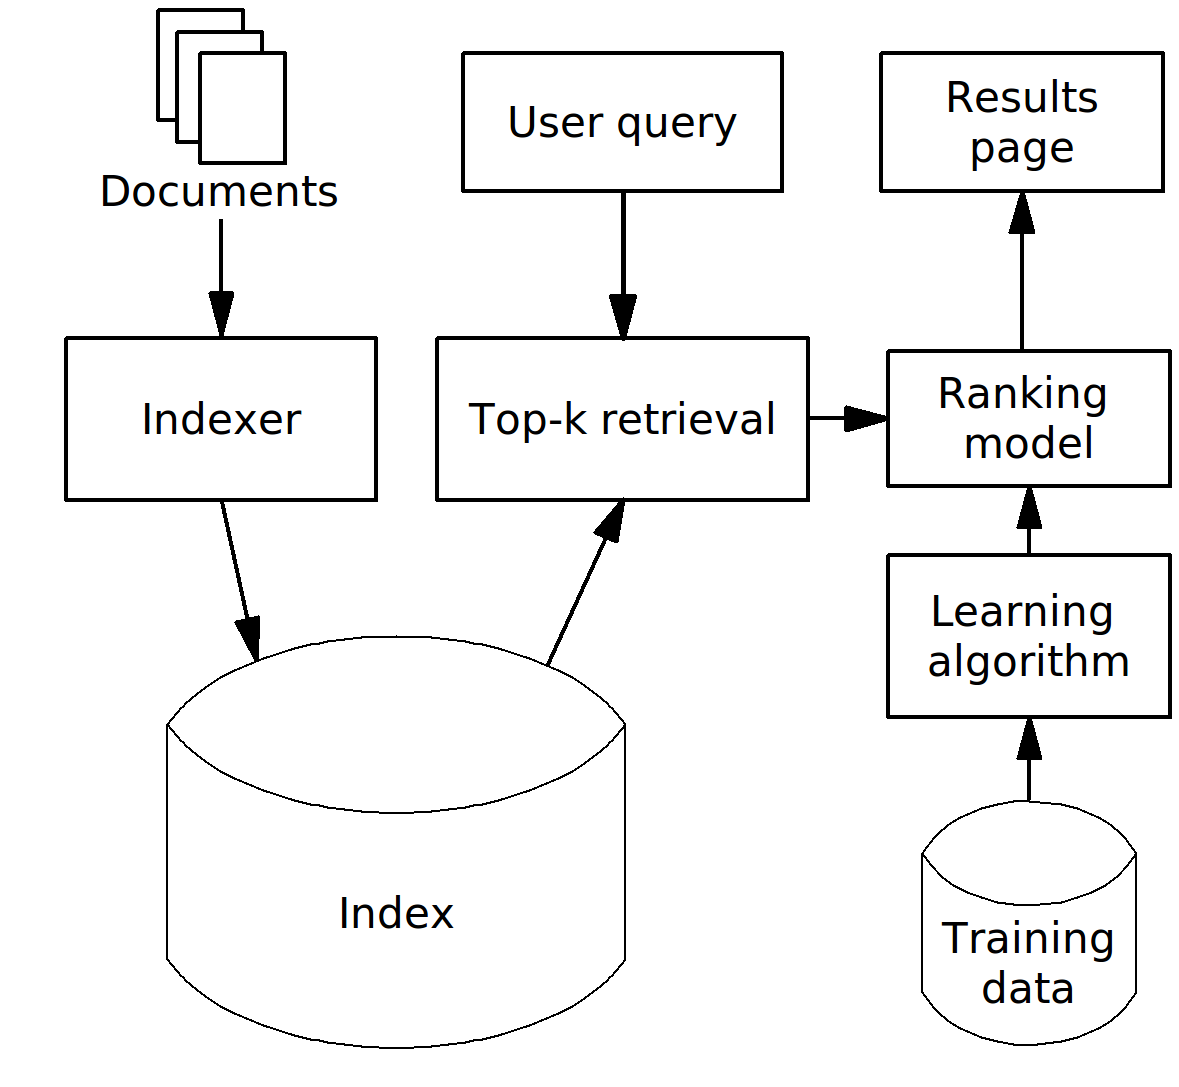
\includegraphics[width=0.5\textwidth]{readme.assets/image-20231223172059132.png}
\caption{The Pipeline of a Typical Learning-to-Rank System \cite{c3}}
\label{l2r pipeline}
\end{figure}

One approach, learning-to-rank, employs machine learning models to
understand relevance beyond keyword matching. Instead of using only one
function, such as BM25, it employs more features extracted from queries
and documents to rank documents. A typical system pipeline is shown in
Fig. \ref{l2r pipeline}. There are three approaches to learning-to-rank, namely
pointwise, pairwise, and listwise, which are described in Fig. \ref{l2r approaches} and
Fig. \ref{l2r algorithms}. Although it achieves better results than traditional methods due
to richer representations of queries and documents, it usually needs
manual feature engineering that may need domain knowledge, is
time-consuming, and might not capture intricate semantic relationships
between words and phrases effectively. Learning from handcrafted
features potentially limits the model's ability to handle complex
language nuances.

\begin{figure}[!h]
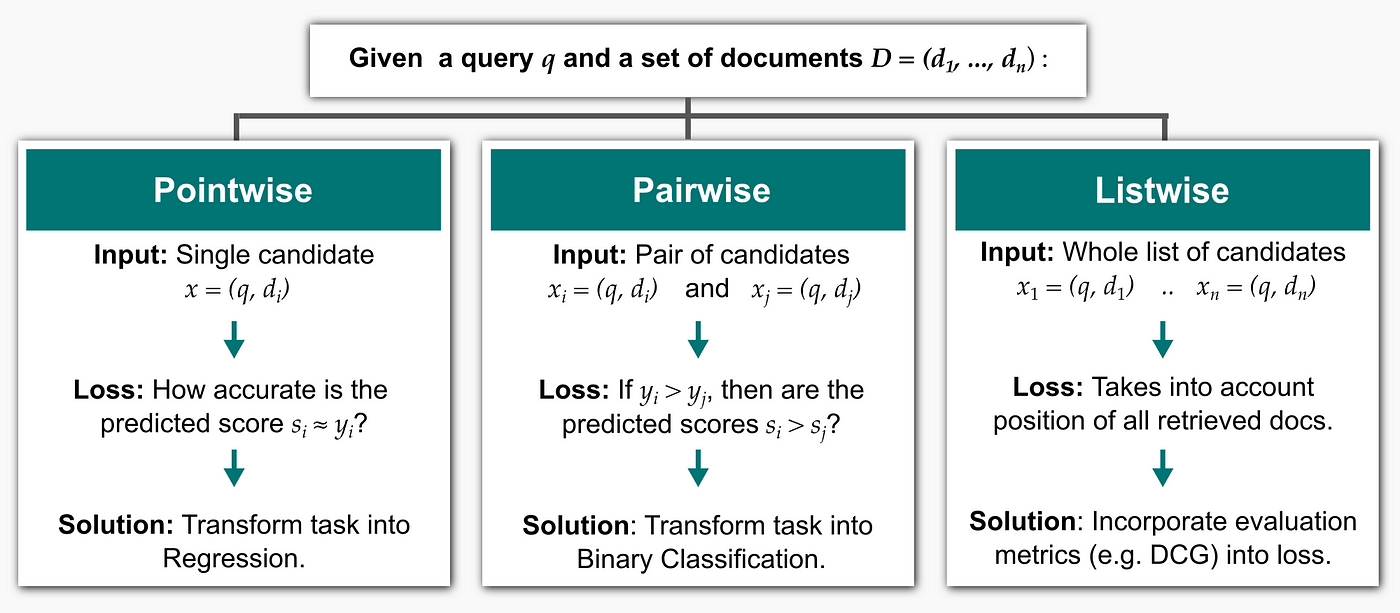
\includegraphics{readme.assets/1s3CQuNRWcQNkQKd8Met-MA.png}
\caption{Three Approaches to Learning-to-Rank \cite{c4}}
\label{l2r approaches}
\end{figure}

\begin{figure}[!h]
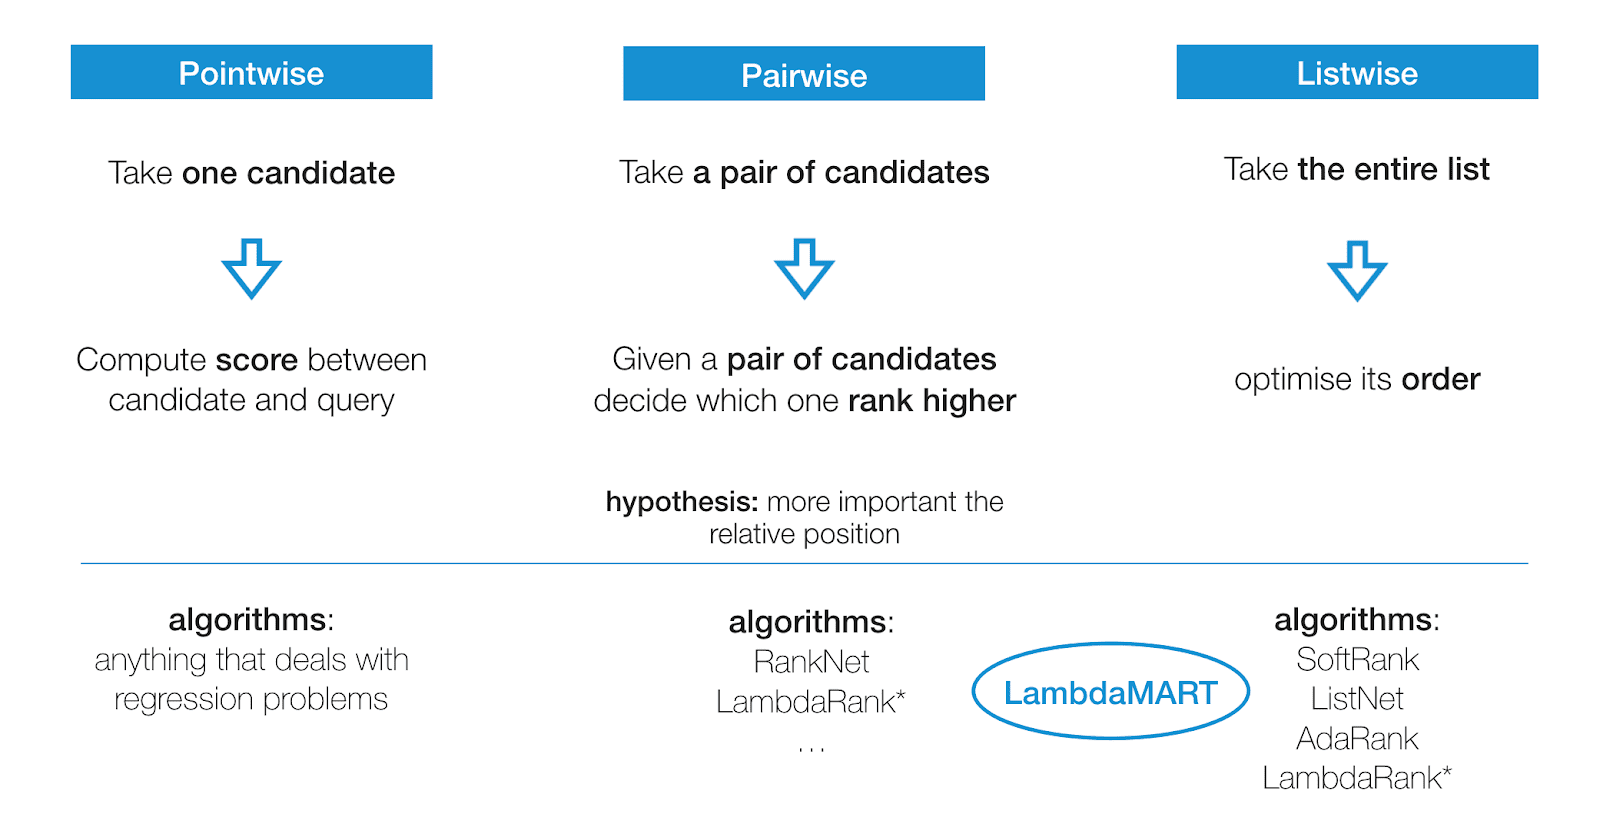
\includegraphics{readme.assets/list_wise_lucidworks.png}
\caption{Algorithms for Three Approaches to Learning-to-Rank \cite{c5}}
\label{l2r algorithms}
\end{figure}

A notable evolution has come through Transformer-based methods.
Transformers, due to their attention mechanisms, excel at converting
queries and documents into dense semantic embeddings that capture their
meaning and context effectively and automatically, alleviating the need
for manual feature engineering and potentially capturing more nuanced
relationships in the data. In addition, pre-trained models can leverage
transfer learning, benefiting from pre-existing knowledge learned from
large-scale datasets. This capability reduces the dependency on
domain-specific labeled data for achieving good performance. The
pipeline is shown in Fig. \ref{semantic search pipeline}.

\begin{figure}
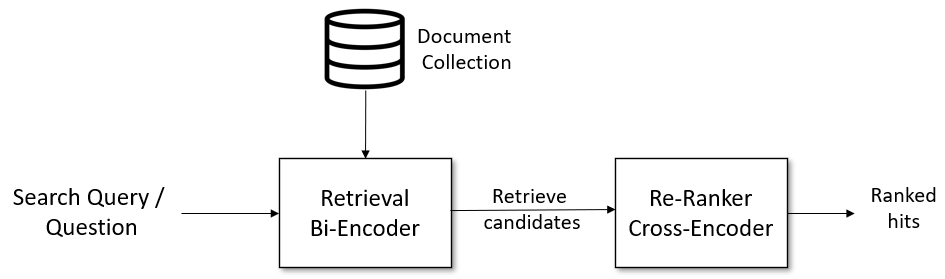
\includegraphics{readme.assets/InformationRetrieval.png}
\caption{The Pipeline of Transformer-based Semantic Search and Re-ranking \cite{c6}}
\label{semantic search pipeline}
\end{figure}

Considering the above, we choose Transformer-based methods. The main
achievements of this project are as follows:

\begin{itemize}
\item
  Utilized Transformer-based models to implement semantic search on the
  MS MARCO dataset.
\item
  Measured and compared the performance of the Transformer-based
  approach and the traditional BM25 algorithm using search quality
  metrics, demonstrating the effectiveness of Transformer-based semantic
  search.
\item
  Seamlessly integrated the Transformer-based semantic search into the
  search engine developed in previous assignments while achieving good
  real-time search efficiency.
\end{itemize}

\hypertarget{ii-method}{%
\section{II. Method}\label{ii-method}}

\hypertarget{1-semantic-search}{%
\subsection{1. Semantic Search}\label{1-semantic-search}}

Semantic search seeks to improve search accuracy by understanding the
content of the search query. In contrast to traditional methods that
only find documents based on lexical matches, semantic search can also
find synonyms. The idea is to embed all documents into a corpus vector
space. At search time, the query is embedded into the same vector space,
and the closest embeddings from the corpus can be found using the cosine
similarity since the embeddings are fixed-sized. These entries should
have a high semantic overlap with the query. The principle is
illustrated in Fig. \ref{semantic search principle}.

\begin{figure}
\centering
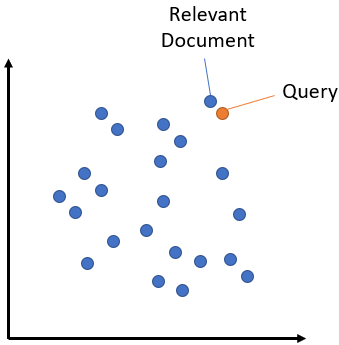
\includegraphics[width=0.4\textwidth]{readme.assets/SemanticSearch.png}
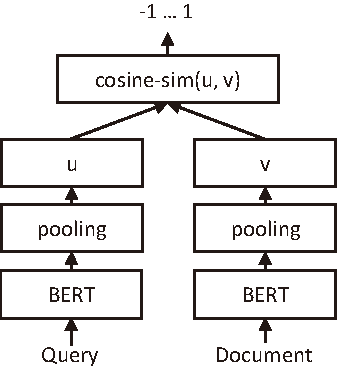
\includegraphics{readme.assets/bi-encoder.pdf}
\caption{The Principle of Semantic Search \cite{c7}}
\label{semantic search principle}
\end{figure}

Recall that in Fig. \ref{semantic search pipeline}, there is no index like Fig. \ref{l2r pipeline}. This is because we
do not match words anymore; instead, all documents in the dataset are
transformed into corpus embeddings. The embeddings are just like the
indexes of documents. The Transformer is usually called a bi-encoder.

\hypertarget{2-reranking}{%
\subsection{2. Reranking}\label{2-reranking}}

The bi-encoder might return irrelevant candidates. A re-ranker based on
a cross-encoder may improve the final results for the user, as it
performs attention across the query and the document---the query and a
possible document are passed simultaneously to Transformer network,
which then outputs a single score between 0 and 1 indicating how
relevant the document is for the given query, as shown in Fig. \ref{reranking principle}.
Scoring millions of (query, document)-pairs would be rather slow; it is
only suitable for reranking a small set of passages. Hence, we can use
the bi-encoder to create a set of (e.g., 32) possible candidates, which
are then reranked by the cross-encoder so that the most relevant
passages are at the top of the result list.

\begin{figure}
\centering
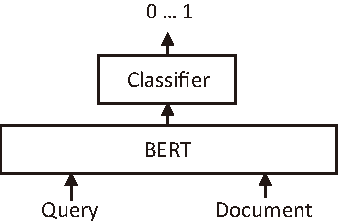
\includegraphics{readme.assets/cross-encoder.pdf}
\caption{The Principle of Reranking}
\label{reranking principle}
\end{figure}

\hypertarget{iii-implementation-and-experiment}{%
\section{III. Implementation and
Experiment}\label{iii-implementation-and-experiment}}

\hypertarget{1-platform-dataset-and-metrics}{%
\subsection{1. Platform, Dataset, and
Metrics}\label{1-platform-dataset-and-metrics}}

The computational platform is the newest laptop with an Intel i9-13900H
CPU (14 cores, 20 threads, up to 5.4 GHz), 48 GB RAM, and an 8 GB NVIDIA
4060 GPU (up to 140 Watt).

The MS MARCO document ranking dataset contains 367013 queries and 384597
ground truths of relevance. There are 12014 empty documents, so the
number of valid ones is 3201821.

Since the relevance ground truth only includes true/false values, the
Mean Reciprocal Rank (MRR) is used to measure the search quality. Let
\(r_i\) be the document rank of the \(i\)th query,

\begin{equation}
\text{MRR} = \frac{1}{n} \sum_{i = 1}^{n} \frac{1}{r_i}.
\end{equation}

Since only 10 documents for each query are returned, if the relevant
document is not in the first 10 results, the reciprocal rank of that
query is recorded as 0.

\hypertarget{2-bm25-baseline}{%
\subsection{2. BM25 Baseline}\label{2-bm25-baseline}}

Since there is no thread pool in the standard library of C++, it is
implemented from scratch to leverage multiple cores to benchmark the
performance of BM25. Mutexes and condition variables are used to
distribute tasks to worker threads safely and save results in the daemon
thread. A cache is also implemented to boost the evaluation speed, and
all classes are designed to be thread-safe to produce reliable results.

The experiment was performed on Linux because of its higher code
execution efficiency. It took 7 minutes and 40 seconds to evaluate the
performance of the whole dataset, with an MRR@10 of 0.153. It reproduces
the official result \cite{c8}, showing the correctness of the implementation.

\begin{figure}
\includegraphics{readme.assets/Screenshot 2023-12-24 022232.png}
\caption{Irrelevant Results of BM25}
\label{bm25 results}
\end{figure}

\hypertarget{3-semantic-search}{%
\subsection{3. Semantic Search}\label{3-semantic-search}}

Due to time and laptop resource constraints, it is infeasible to train Transformers from scratch, so pre-trained models have to be used. The \texttt{sentence\_transformer} package provides several pre-trained models and utilities suitable for this task. The model is called SBERT \cite{c9}, which contains a pooling layer after the output of BERT / RoBERTa, enabling it to derive a fixed-sized sentence embedding. The bi-encoder model \texttt{multi-qa-MiniLM-L6-cos-v1} and \texttt{msmarco-MiniLM-L6-cos-v5} are tried for semantic search, which both map sentences and paragraphs to a 384-dimensional dense vector space. The former has been trained on 215M question-answer pairs from various sources and domains and performs well across many search tasks and domains. The latter has been trained on 500K (query, answer) pairs from the MS MARCO dataset. They are the fastest models provided by the package. \cite{c10}

To allow memory for subsequent queries, we truncate long articles to 256 tokens. It took 2 hours to generate embeddings of all documents, which is 4.58 GB. Interestingly, the non-compressed binary index created in previous assignments is 4.69 GB, roughly the same size as the embeddings. Generating embeddings for all documents does not require much GPU memory; if the batch size is set to be too large, it may take longer, and the CPU/GPU may not be fully utilized. Evaluating the models' performance on the entire dataset took less than 9 minutes and consumed 7 GB of GPU memory. The \texttt{multi-qa-MiniLM-L6-cos-v1} model achieves an MRR@10 of 0.292, and the \texttt{msmarco-MiniLM-L6-cos-v5} model achieves an MRR@10 of 0.315, more than twice that of BM25, showing the effectiveness of the Transformer-based semantic search.

Fig. \ref{semantic search results} is the result using the \texttt{multi-qa-MiniLM-L6-cos-v1} model.
Intuitively, the comparison between Fig. \ref{semantic search results} and
Fig. \ref{bm25 results} shows the semantic
search results are indeed more relevant than BM25. Although the semantic
results in Fig. \ref{semantic search results} do not contain the query word ``essence," the content
is very relevant to the query. On the contrary, the BM25 results in Fig.
8 suffer from BM25's assumption that a scarce word should receive higher
weights---although ``essence" has the highest frequency in the first
passage, it is totally irrelevant to the query, thus highlighting the
importance of semantic understanding.

\hypertarget{4-reranking}{%
\subsection{4. Reranking}\label{4-reranking}}

The cross-encoder model \texttt{ms-marco-MiniLM-L-6-v2} is used for
reranking the results from the semantic search because it has a higher
MRR than the \texttt{L-4} version and is only 0.0001 lower but much
faster than the \texttt{L-12} version MRR. It took 15 hours on Linux to
evaluate the performance of the whole dataset, consuming 8 GB of GPU
memory and 110 W of GPU power with a batch size of 224. The model
achieves an MRR@10 of 0.173, which is unexpectedly lower than the
semantic search result of the \texttt{multi-qa-MiniLM-L6-cos-v1} model 
and the result claimed for the \texttt{dev}
dataset of MS MARCO. The likely reason for this is that in the current
implementation, excessively long articles are automatically truncated by
the model, which produces inaccurate results. One possible improvement
is to split long articles with an overlapping window and to take only
the maximum value for paragraphs belonging to the same article during
retrieval. The first passage in the search results shown in Fig. \ref{reranking results} also
seems not so relevant to the query, but it is much better than the
purely irrelevant results of BM25.

\begin{figure}
\includegraphics{readme.assets/Screenshot 2023-12-24 021938.png}
\caption{Results of Reranking}
\label{reranking results}
\end{figure}

\hypertarget{5-integration}{%
\subsection{5. Integration}\label{5-integration}}

Since the \texttt{sentence\_transformer} package is on Python,
integration needs to call Python code from C++ using the CPython C API.
Memory management requires special attention and effort, and various
cases that require \texttt{INCREF}, \texttt{DECREF}, and those that do
not need \texttt{INCREF} or \texttt{DECREF} due to built-in objects
``stealing" references are well considered to prevent memory leaks.
Besides, in the web mode, the system has multiple threads, preventing
the Python interpreter acquiring the Global Interpreter Lock (GIL).
Thus, we use
\texttt{Py\_BEGIN\_ALLOW\_THREADS\ auto\ gstate\ =\ PyGILState\_Ensure();}
and \texttt{PyGILState\_Release(gstate);\ Py\_END\_ALLOW\_THREADS} to
force the interpreter to execute Python code while there are other
non-Python threads running. New queries can be executed typically in
hundreds of milliseconds, as shown in Fig. \ref{semantic search results} and Fig. \ref{reranking results}, demonstrating
good efficiency.

\hypertarget{iv-conclusion}{%
\section{IV. Conclusion}\label{iv-conclusion}}

In this project, the Transformer-based semantic search approach is
employed to improve the search quality on the MS MARCO dataset.
Comparative experiments show that semantic search achieves better
relevance than BM25. Semantic search is also integrated into the search
engine developed in previous assignments, making it more powerful while
remaining efficient. In the future, we can ensemble more
state-of-the-art methods or propose new approaches to boost its
performance. By researching, designing, and implementing the search
engine, the author has gained a deeper understanding and a broader
perspective on web search engines and information retrieval, as well as
practical skills for similar tasks.

\hypertarget{appendix}{%
\section{Appendix}\label{appendix}}

\hypertarget{1-file-description}{%
\subsection{1. File Description}\label{1-file-description}}

\hypertarget{a-convertidscpp}{%
\subsubsection{a.
\texttt{convert\_ids.cpp}}\label{a-convertidscpp}}

This file converts raw document IDs in the MS MARCO dataset to numerical
IDs used in other programs. It calls Win32 API to use memory maps to
parse the dataset efficiently.

\begin{Shaded}
\begin{Highlighting}[]
\ExtensionTok{Usage:}\NormalTok{ ./convert\_ids [{-}h] [{-}d dataset\_file\_path]
}
\ExtensionTok{Options:
}
        \ExtensionTok{{-}d}\NormalTok{      dataset path, default: fulldocs{-}new.trec
}
        \ExtensionTok{{-}h}\NormalTok{      help}
\end{Highlighting}
\end{Shaded}

\hypertarget{b-evaluationcpp}{%
\subsubsection{b.
\texttt{evaluation.cpp}}\label{b-evaluationcpp}}

This file evaluates MRR@10 of BM25 on the whole dataset. It uses all
logical cores by default.

\begin{Shaded}
\begin{Highlighting}[]
\ExtensionTok{Usage:}\NormalTok{ ./evaluation [{-}h] [{-}p doc\_info\_file] [{-}s storage\_info\_file]
}
    \ExtensionTok{[{-}i}\NormalTok{ index\_ids\_file] [{-}f index\_freqs\_file] [{-}t index\_file\_type]
}
    \ExtensionTok{[{-}q}\NormalTok{ queries\_path] [{-}r relevance\_path] [{-}n n\_results] [{-}m n\_threads]
}
    \ExtensionTok{[{-}c}\NormalTok{ cache\_size]
}
\ExtensionTok{Options:
}
    \ExtensionTok{{-}p}\NormalTok{      doc info }\ErrorTok{(}\ExtensionTok{page}\NormalTok{ table}\KeywordTok{)} \FunctionTok{file}\NormalTok{, default: docs.txt
}
    \ExtensionTok{{-}s}\NormalTok{      storage info }\ErrorTok{(}\ExtensionTok{lexicon}\KeywordTok{)} \FunctionTok{file}\NormalTok{, default: storage\_vbyte.txt
}
    \ExtensionTok{{-}i}\NormalTok{      index ids file, default: merged\_index.vbyte
}
    \ExtensionTok{{-}f}\NormalTok{      index freqs file, default: freqs.vbyte
}
    \ExtensionTok{{-}t}\NormalTok{      index file type }\ErrorTok{(}\ExtensionTok{bin}\KeywordTok{|}\ExtensionTok{vbyte}\KeywordTok{)}\ExtensionTok{,}\NormalTok{ default: vbyte
}
    \ExtensionTok{{-}q}\NormalTok{      queries path, default: queries.doctrain.tsv
}
    \ExtensionTok{{-}r}\NormalTok{      relevance path, default: msmarco{-}doctrain{-}qrels{-}idconverted.tsv
}
    \ExtensionTok{{-}n}\NormalTok{      number of results, default: 10
}
    \ExtensionTok{{-}m}\NormalTok{      number of threads, default: number of logical cores
}
            \KeywordTok{(}\ExtensionTok{20}\NormalTok{ on this machine}\KeywordTok{)}
    \ExtensionTok{{-}c}\NormalTok{      cache size, default: 131072
}
    \ExtensionTok{{-}h}\NormalTok{      help}
\end{Highlighting}
\end{Shaded}        

\hypertarget{c-saveembeddingsipynb}{%
\subsubsection{c.
\texttt{save\_embeddings.ipynb}}\label{c-saveembeddingsipynb}}

This file is a Jupyter Notebook for saving corpus embeddings of all
documents. It also generates the \texttt{corpus\_id\_to\_doc\_id.txt}
file because empty documents are removed in the embeddings; thus, new
corpus IDs are formed, but they are not removed during indexing, so it
will be needed to look up document IDs according to corpus IDs. It loads
the whole dataset into the memory, so at least 64 GB of memory is
required to avoid memory swapping.

\hypertarget{d-evalsemanticsearchipynb}{%
\subsubsection{d.
\texttt{eval\_semantic\_search.ipynb}}\label{d-evalsemanticsearchipynb}}

This file is a Jupyter Notebook for evaluating the semantic search
performance on the whole dataset.

\hypertarget{e-evalrerankipynb}{%
\subsubsection{e.
\texttt{eval\_rerank.ipynb}}\label{e-evalrerankipynb}}

This file is a Jupyter Notebook for evaluating the performance of
reranking on the whole dataset.

\hypertarget{c-learningtorankpy}{%
\subsubsection{c. \texttt{learning\_to\_rank.py} (although
it is not the learning-to-rank mentioned
above)}\label{c-learningtorankpy}}

This file is a Python script that loads the bi-encoder, cross-encoder,
and corpus embeddings, and contains the \texttt{semantic\_search} and
the \texttt{rerank\_inplace} functions. Default values including
\texttt{device\ =\ \textquotesingle{}cuda\textquotesingle{}\ if\ torch.cuda.is\_available()\ else\ \textquotesingle{}cpu\textquotesingle{}},
\texttt{bi\_encoder.max\_seq\_length\ =\ 256}, \texttt{top\_k\ =\ 32}
and \texttt{corpus\_embeddings.pt} can be modified directly from this
file. It maps \texttt{corpus\_embeddings.pt} directly to the memory that
GPU can access, avoiding the overhead of copying the data from the disk
to the main memory at first when using the CUDA backend. However, the
file name and function signature cannot be modified without also
modifying the \texttt{main.cpp} file.

\hypertarget{d-maincpp-and-the-indexhtml-web-page}{%
\subsubsection{d. \texttt{main.cpp} and the
\texttt{index.html} web page}\label{d-maincpp-and-the-indexhtml-web-page}}

\texttt{main.exe} reads the page table and the lexicon into the memory
and waits for input from the user.

\emph{\textbf{For BM25-Based Retrieval.}} After receiving the user's
query, it cleans it, removing leading and trailing blanks and repeated
terms, and converts ascii letters to lowercase letters. Then, it checks
if the query result is in the cache. If it is, it returns the cached
result. Otherwise, it checks if each term's index entry is in the cache.
If not, it gets the storage information from the lexicon and reads
entries of query terms from the index file. After that, it selects
documents based on the query type, conjunctive and disjunctive. Since
\texttt{docID}s are sorted, conjunctive query intersects \texttt{docID}s
in \(O(n)\) time, and disjunctive query unions \texttt{docID}s also in
\(O(n)\) time. Then, it calculates the ranking score of the selected
documents using BM25 and sorts them based on the score. The
consideration here is the same as \texttt{create\_index}.

\emph{\textbf{For Transformer-Based Retrieval.}} After receiving the
user's query, it checks if the query result is in the cache. If it is,
it returns the cached result. Otherwise, it calls the Python function to
perform semantic search. If the query type is \texttt{RERANKING}, it
then calls the Python function to perform reranking.

After that, it caches the result and generates snippets of the result.
It seeks the dataset according to the information in the page table,
tokenizes the document, finds the first occurrence of one of the query
terms, and expands the start and end positions of the snippet according
to this position. Since the snippet length can be changed via the web
API, there is no point in caching snippets. Finally, it returns the
results to the web or the terminal. During the entire process, pointers
are used to avoid copying arrays for efficiency.

The single-header library \texttt{httplib.h} is used for the program to
become a web server. The server responds with \texttt{index.html} for
HTTP GET requests and JSON for HTTP POST requests to the root. The
server is robust to bad requests, including malformed JSON, missing
properties, type-mismatch, invalid values, etc. In \texttt{index.html},
Bootstrap is used to build the responsive UI, and \texttt{axios} is used
to send asynchronized HTTP POST requests to the server. Results are
dynamically added to the page using JavaScript.

An example of the JSON sent from the web is shown as follows:

\begin{Shaded}
\begin{Highlighting}[]
\FunctionTok{\{}
    \DataTypeTok{"query"}\FunctionTok{:} \StringTok{"\textless{}query words\textgreater{}"}\FunctionTok{,}
    \DataTypeTok{"query\_type"}\FunctionTok{:} \DecValTok{1}\FunctionTok{,}
    \ErrorTok{//} \ErrorTok{1}\FunctionTok{:} \ErrorTok{conjunctive}\FunctionTok{,} \ErrorTok{2}\FunctionTok{:} \ErrorTok{disjunctive}\FunctionTok{,} \ErrorTok{3}\FunctionTok{:} \ErrorTok{semantic}\FunctionTok{,} \ErrorTok{4}\FunctionTok{:} \ErrorTok{reranking}
    \StringTok{"n\_results"}\ErrorTok{:} \DecValTok{10}\FunctionTok{,}
    \DataTypeTok{"snippet\_len"}\FunctionTok{:} \DecValTok{200}
\FunctionTok{\}}
\end{Highlighting}
\end{Shaded}

An example of a successful query of the JSON returned from the server is
shown as follows:

\begin{Shaded}
\begin{Highlighting}[]
\FunctionTok{\{}
    \DataTypeTok{"cached"}\FunctionTok{:} \KeywordTok{true}\FunctionTok{,}
    \DataTypeTok{"time"}\FunctionTok{:} \DecValTok{1}\FunctionTok{,} \ErrorTok{//} \ErrorTok{in} \ErrorTok{microseconds}
    \DataTypeTok{"count"}\FunctionTok{:} \DecValTok{10000}\FunctionTok{,}
    \DataTypeTok{"data"}\FunctionTok{:} \OtherTok{[}
    \FunctionTok{\{}
        \DataTypeTok{"rank"}\FunctionTok{:} \DecValTok{1}\FunctionTok{,}
        \DataTypeTok{"score"}\FunctionTok{:} \FloatTok{7.6}\FunctionTok{,}
        \DataTypeTok{"freqs"}\FunctionTok{:} \OtherTok{[[}\StringTok{"\textless{}a query word\textgreater{}"}\OtherTok{,} \DecValTok{1000}\OtherTok{],} \ErrorTok{/*...*/}\OtherTok{]}\FunctionTok{,}
        \ErrorTok{//} \ErrorTok{only} \ErrorTok{BM25{-}based} \ErrorTok{retrieval} \ErrorTok{has} \ErrorTok{this} \ErrorTok{field}
        \DataTypeTok{"url"}\FunctionTok{:} \StringTok{"\textless{}url\textgreater{}"}
        \StringTok{"snippet"}\ErrorTok{:} \StringTok{"\textless{}snippet\textgreater{}"}
    \FunctionTok{\}}\OtherTok{,} \ErrorTok{//} \ErrorTok{...}
    \OtherTok{]}
\FunctionTok{\}}
\end{Highlighting}
\end{Shaded}

\texttt{learning\_to\_rank.py} must be located in the current working
directory of \texttt{main.exe}. On Windows, \texttt{python3xx.dll} must
be in the \texttt{PATH} environment variable. On Linux,
\texttt{libpython3xx.so} must be in the \texttt{LD\_LIBRARY\_PATH}. The
linked Python environment must have \texttt{sentence\_transformer}
installed, which can be installed using
\texttt{pip\ install\ sentence\_transformer}.

\begin{Shaded}
\begin{Highlighting}[]
\ExtensionTok{Usage:}\NormalTok{ ./main [{-}h] [{-}d dataset\_file] [{-}p doc\_info\_file] [{-}s storage\_info\_file]
}
    \ExtensionTok{[{-}i}\NormalTok{ index\_ids\_file] [{-}f index\_freqs\_file] [{-}t index\_file\_type]
}
    \ExtensionTok{[{-}c}\NormalTok{ corpus\_id\_to\_doc\_id\_file] [{-}w server\_port] [{-}q query\_type]
}
    \ExtensionTok{[{-}n}\NormalTok{ n\_results] [{-}l snippet\_len] [{-}m cache\_size]
}
\ExtensionTok{Options:
}
    \ExtensionTok{{-}d}\NormalTok{      dataset file, default: fulldocs{-}new.trec
}
    \ExtensionTok{{-}p}\NormalTok{      doc info }\ErrorTok{(}\ExtensionTok{page}\NormalTok{ table}\KeywordTok{)} \FunctionTok{file}\NormalTok{, default: docs.txt
}
    \ExtensionTok{{-}s}\NormalTok{      storage info }\ErrorTok{(}\ExtensionTok{lexicon}\KeywordTok{)} \FunctionTok{file}\NormalTok{, default: storage\_vbyte.txt
}
    \ExtensionTok{{-}i}\NormalTok{      index ids file, default: merged\_index.vbyte
}
    \ExtensionTok{{-}f}\NormalTok{      index freqs file, default: freqs.vbyte
}
    \ExtensionTok{{-}t}\NormalTok{      index file type }\ErrorTok{(}\ExtensionTok{bin}\KeywordTok{|}\ExtensionTok{vbyte}\KeywordTok{)}\ExtensionTok{,}\NormalTok{ default: vbyte
}
    \ExtensionTok{{-}c}\NormalTok{      corpus id to doc id file, default: corpus\_id\_to\_doc\_id.txt
}
    \ExtensionTok{{-}w}\NormalTok{      server port }\ErrorTok{(}\ExtensionTok{[0,}\NormalTok{ 65535] for web, others for cli}\KeywordTok{)}\ExtensionTok{,}\NormalTok{ default: 8080
}
    \ExtensionTok{{-}q}\NormalTok{      query type for cli }\ErrorTok{(}\ExtensionTok{conjunctive}\KeywordTok{|}\ExtensionTok{disjunctive}\KeywordTok{|}\ExtensionTok{semantic}\KeywordTok{|}\ExtensionTok{reranking}\KeywordTok{)}\ExtensionTok{,
}
            \ExtensionTok{default:}\NormalTok{ semantic
}
    \ExtensionTok{{-}n}\NormalTok{      number of results, default: 10
}
    \ExtensionTok{{-}l}\NormalTok{      snippet length, default: 200
}
    \ExtensionTok{{-}m}\NormalTok{      cache size, default: 1000
}
    \ExtensionTok{{-}h}\NormalTok{      help}
\end{Highlighting}
\end{Shaded}
        
\hypertarget{2-limitations}{%
\subsection{2. Limitations}\label{2-limitations}}

\begin{itemize}
\item
  Other models trained using multi-language sources are needed to
  support multi-language.
\item
  The web server is not designed to receive concurrent queries. This
  decision keeps the program lightweight.
\end{itemize}

\begin{thebibliography}{99}

\bibitem{c1}S. E. Robertson, S. Walker, S. Jones, M. Hancock-Beaulieu, and M. Gatford. Okapi at TREC-3.
\bibitem{c2}A. Trotman, X-F. Jia, and M. Crane. Towards an efficient and effective search engine.
\bibitem{c3}\href{https://www.cl.cam.ac.uk/teaching/1516/R222/l2r-overview.pdf}{R. Cummins and T. Briscoe. Learning to Rank.}
\bibitem{c4}\href{https://miro.medium.com/v2/resize:fit:1400/format:webp/1*s3CQuNRWcQNkQKd8Met-MA.png}{F. Casalegno. Learning to Rank: A Complete Guide to Ranking using Machine Learning.}
\bibitem{c5}\href{https://lucidworks.com/wp-content/uploads/2019/11/list_wise_lucidworks.png}{J. Le. The ABCs of Learning to Rank.}
\bibitem{c6}\href{https://raw.githubusercontent.com/UKPLab/sentence-transformers/master/docs/img/InformationRetrieval.png}{sbert.net}
\bibitem{c7}\href{https://raw.githubusercontent.com/UKPLab/sentence-transformers/master/docs/img/SemanticSearch.png}{sbert.net}
\bibitem{c8}N. Craswell, B. Mitra, E. Yilmaz, D. Campos, and J. Lin. MS MARCO: Benchmarking Ranking Models in the Large-Data Regime.
\bibitem{c9}N. Reimers and I. Gurevych. Sentence-BERT: Sentence Embeddings using Siamese BERT-Networks.
\bibitem{c10}\href{https://www.sbert.net/docs/pretrained_models.html}{Pretrained Models --- Sentence-Transformers documentation (sbert.net)}

\end{thebibliography}

\end{document}
